\begin{figure}
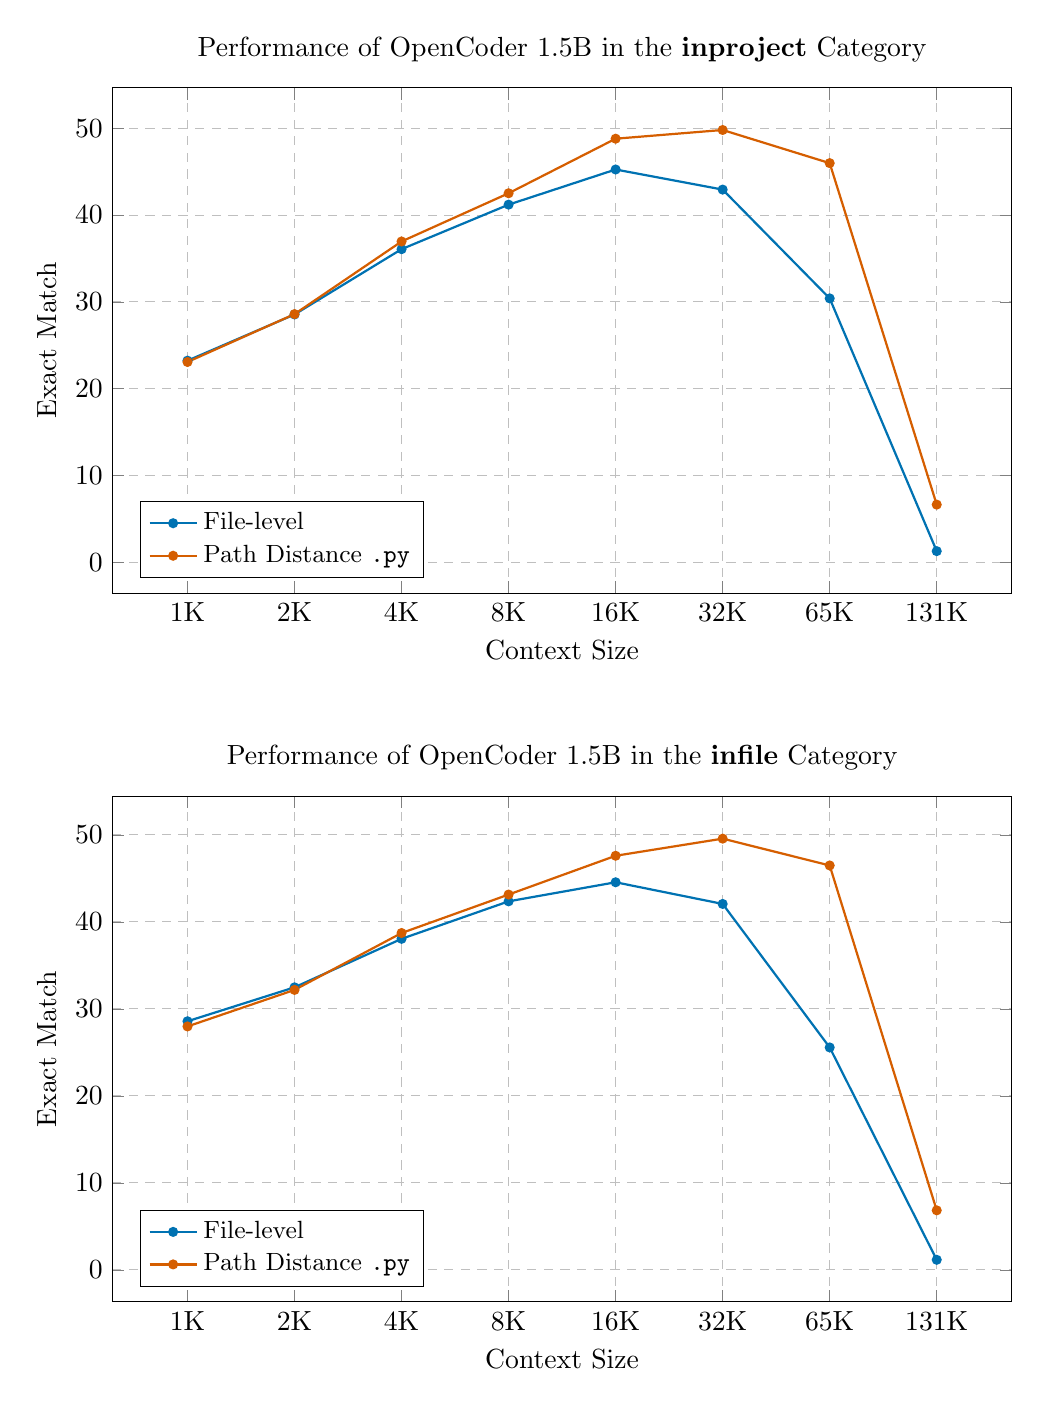
\begin{tikzpicture}

\definecolor{custom_blue}{RGB}{0, 114, 178}
\definecolor{custom_orange}{RGB}{213, 94, 0}

% inproject
\begin{axis}[
    xlabel=Context Size,
    ylabel=Exact Match,
    xmode=log,
    log basis x=2,
    grid=major,
    grid style={dashed, line width=0.0pt},
    legend pos=south west,
    width=13cm,
    height=8cm,
    at={(0,9cm)},
    xtick={1024,2048,4096,8192,16384,32768,65536,131072},
    xticklabels={1K,2K,4K,8K,16K,32K,65K,131K},
    legend style={font=\small},
    legend cell align={left},
    title=Performance of OpenCoder 1.5B in the \textbf{inproject} Category
]
% File-level
\addplot[
    color=custom_blue,
    mark=*,
    mark options={
        scale=0.7,
    },
    thick,
] coordinates {
    (1024,23.236994)
    (2048,28.554913)
    (4096,36.069364)
    (8192,41.194605)
    (16384,45.240848)
    (32768,42.928709)
    (65536,30.404624)
    (131072,1.310212)
};

% Baseline
\addplot[
    color=custom_orange,
    mark=*,
    mark options={
        scale=0.7,
    },
    thick,
] coordinates {
    (1024,23.082852)
    (2048,28.593449)
    (4096,36.955684)
    (8192,42.504817)
    (16384,48.786127)
    (32768,49.788054)
    (65536,45.973025)
    (131072,6.666667)
};
\legend{
    {File-level},
    {Path Distance \texttt{.py}}
}
\end{axis}

% infile
\begin{axis}[
    xlabel=Context Size,
    ylabel=Exact Match,
    xmode=log,
    log basis x=2,
    grid=major,
    grid style={dashed, line width=0.0pt},
    legend pos=south west,
    width=13cm,
    height=8cm,
    xtick={1024,2048,4096,8192,16384,32768,65536,131072},
    xticklabels={1K,2K,4K,8K,16K,32K,65K,131K},
    legend style={font=\small},
    legend cell align={left},
    title=Performance of OpenCoder 1.5B in the \textbf{infile} Category
]
% File-level
\addplot[
    color=custom_blue,
    mark=*,
    mark options={
        scale=0.7,
    },
    thick,
] coordinates {
    (1024,28.576737)
    (2048,32.478632)
    (4096,38.052768)
    (8192,42.363434)
    (16384,44.555927)
    (32768,42.066146)
    (65536,25.566704)
    (131072,1.151988)
};

% Baseline
\addplot[
    color=custom_orange,
    mark=*,
    mark options={
        scale=0.7,
    },
    thick,
] coordinates {
    (1024,27.982163)
    (2048,32.181345)
    (4096,38.721665)
    (8192,43.143813)
    (16384,47.603122)
    (32768,49.572650)
    (65536,46.488294)
    (131072,6.837607)
};
\legend{
    {File-level},
    {Path Distance \texttt{.py}}
}
\end{axis}
\end{tikzpicture}

\caption{Performance comparison of File-level and Path Distance \texttt{.py} approaches across different context sizes for OpenCoder 1.5B model. The plots show the Exact Match accuracy for both inproject (top) and infile (bottom) categories.}
\label{fig:beyound_training_context_window}
\end{figure}
